%\section{Approcci}
% Prima di addentrarci nella discussione dei risultati è bene introdurre le
% modalità con cui si sono svolti gli esperimenti.\\
% Dal punto di vista dei linguaggi di programmazione si sono usati:
% \begin{itemize}
%   \item \textbf{\Cplusplus}, per l'implementazione delle strutture dati e degli
%   algoritmi
%   \item \textbf{Python}, per la creazione della struttura a partire dal
%   pannello in input e per gestire l'intera pipeline di sperimentazione,
%   partendo dal \textit{preprocessing} dell'input fino alla produzione dei
%   grafici al termine della computazione
% \end{itemize}
% Nel dettaglio la costruzione della \textbf{RLPBWT}, i cui
% singoli step verranno approfonditi nel corso del capitolo, si articola nel
% seguente modo: 
% \begin{enumerate}
%   \item \textit{\textbf{input:}} pannello binario generato tramite
%   \textbf{MaCS} oppure un pannello in \textbf{Variant Call Format (VCF)}
%   \cite{vcf}, nel 
%   caso di dati reali, convertito per praticità in formato \textit{MACs}
%   \item \textbf{opzionale:} produzione dell'\textbf{SLP} del pannello
%   \item \textbf{step intermedio:} estrazione dal pannello in input di un
%   pannello di query di grandezza selezionata dall'utente e costruzione della
%   struttura dati  
%   \item \textbf{opzionale:} serializzazione della struttura dati, tramite
%   \textbf{SDSL} 
%   \item \textit{\textbf{output:}} file contenente gli \textit{SMEM}
% \end{enumerate}
% Si specifica che per il file di output si è mantenuto lo stesso formato
% utilizzato da Durbin nella sua implementazione della \textbf{PBWT}
% \cite{durbin_gh}. Tale formato prevede, per facilitarne il parsing, un
% \texttt{tsv} (\textit{tab-separated values}) con le seguenti colonne:
% \begin{enumerate}
%   \item colonna semplicemente indicante che si ha uno \textit{SMEM}
%   \item l'indice della query di cui si annota lo \textit{SMEM}
%   \item l'indice dell'aplotipo per cui si ha lo \textit{SMEM}
%   \item l'indice della colonna da cui parte lo \textit{SMEM}
%   \item l'indice della colonna in cui termina lo \textit{SMEM}
%   \item la lunghezza dello \textit{SMEM}
% \end{enumerate}
%Un esempio è visualizzabile alla listing \ref{lst:pbwtres}.
% \paragraph{MaCS}
% \textbf{MaCS} \cite{macs}, sviluppato da Gary K. Chen, è un simulatore di
% \textit{processi coalescenti}, basati sulla \textbf{teoria della
%   coalescenza}. Tale teoria è un modello di come gli alleli campionati da una
% popolazione possano essere originati da un antenato comune. Il tool simula
% genealogie spaziali tra i cromosomi sfruttando processi Markoviani.\\
% Nel dettaglio il lavoro è fortemente ispirato dai risultati di Wiuf e Hein
% \cite{wiuf}, che per primi proposero un algoritmo basato sulla costruzione e
% sulla memorizzazione di un \textbf{ancestral recombination graph
%   (\textit{ARG})}.\\
% Chen stesso segnala le seguenti differenze con l'algoritmo di Wiuf e Hein:
% \begin{itemize}
%   \item gli eventi di ricombinazione si verificano solo sulla geneologia locale
%   nella posizione attuale sulla sequenza invece che in qualsiasi altro punto
%   dell'\textit{ARG}, ma possono unirsi a qualsiasi lignaggio sull'ARG compresi
%   quelli non sulla geneologia locale (ad esempio un arco non ancestrale)
%   \item i tempi di attesa (ovvero la distanza tra le ricombinazioni sulla
%   sequenza) sono calcolati in modo esponenziali con intensità basata sulla
%   lunghezza dell'arco della geneologia locale invece della lunghezza
%   \textit{ARG}
%   \item l''algoritmo è detto dell'$n$-esimo ordine Markoviano, dove $n$ è basato
%   sui parametri inserito dall'utente
% \end{itemize}
% L'autore ricorda che queste modifiche rendono l'algoritmo sostanzialmente più
% efficiente del Wiuf e Hein con poca perdita di precisione. \\
% Dal punto di vista pratico l'esecuzione di \textit{MaCS} produce i pannelli
% binari, da intendersi come pannelli di aplotipi, che verranno poi studiati
% tramite la \textit{PBWT} e la \textit{RLPBWT}. Tali pannelli presentano:
% \begin{itemize}
%   \item un header, con informazioni in merito al comando usato e al seed
%   \item una riga per ogni sito, con prima alcune informazioni in merito a come è
%   stato prodotto il dato e poi la sequenza di valori binari, uno per ogni sample
%   \item un footer, con ulteriori informazioni, tra cui le dimensioni del
%   pannello 
% \end{itemize}
% Quindi, trascurando le varie informazioni aggiuntive, il pannello è
% \textbf{trasposto} rispetto a quanto studiato dalla \textit{PBWT} e dalla
% \textit{RLPBWT}. Questa però risulta essere una comodità in quanto, leggendo
% iterativamente il file, si legge di volta in volta la $i$-esima colonna, ovvero
% quanto serve per la costruzione della struttura dati.\\
% % Per capire meglio come venga prodotto un pannello tramite questo strumento,
% % analizziamo un semplice esempio:
% % \begin{shaded}
% %   \begin{minted}{bash}
% %     ./macs 5 3000 -t 0.001 -r 0.001
% %   \end{minted}
% % \end{shaded}
% % \noindent
% % Dove:
% % \begin{itemize}
% %   \item $5$ è il numero di sample richiesto, ovvero il numero di sequenze che
% %   il software simulerà
% %   \item $3000$ è la lunghezza in paia-basi della regione genomica su cui
% %   verranno simulate le $5$ sequenze
% %   \item \texttt{-t} $0.001$ segnala il \textit{mutation rate} per ogni sito,
% %   ovvero la frequenza di \textit{nuove mutazioni} per un sito nel tempo 
% %   \item \texttt{-r} $0.001$ segnala il \textit{recombination rate} per ogni
% %   sito, ovvero la frequenza di \textit{ricombinazioni geniche}, che sono i
% %   processi per i quali si ottengono nuove combinazioni di alleli a partire da un
% %   \textit{genotipo}, per un sito nel tempo 
% % \end{itemize}
% Tale formato era stato scelto, inizialmente, in quanto scelto da Durbin
% stesso. Avendo, però, deciso di effettuare la sperimentazione su pannelli reali
% si è continuato ad usarne il formato per gli input alle varie strutture per la
% \textit{RLPBWT}, senza effettivamente generare dei pannelli. 
% % Il risultato, dove si noti vengono selezionati 4 siti dopo la simulazione, del
% % comando appena descritto è visualizzabile alla listing \ref{lst:macs}.\\
% % \begin{listing}[H]
% %   \inputminted[obeytabs]{text}{code/example.macs}
% %   \caption{Esempio di output di \textbf{MaCS}.}
% %   \label{lst:macs}
% % \end{listing}
% % \textbf{MANCA SIGNIFICATO DEGLI ``HEADER'' DI OGNI SITE NEL RISULTATO.}
% % \subsection{SDSL}
% % La libreria più utilizzata nel progetto, come anche in diverse sue dipendenze, è
% % \textbf{Succinct Data Structure Library (\textit{SDSL})} \cite{sdsl}. Questa
% % libreria, scritta in \Cplusplus 11, fornisce diverse implementazioni riguardanti
% % strutture dati succinte, come i già citati, nella sezione \ref{bvsec},
% % \textbf{bitvectors}.\\ 
% % Nel dettaglio, in questo progetto, \textit{SDSL} è stata usata per:
% % \begin{itemize}
% %   \item gli \textbf{sparse bitvectors}, il cui uso specifico verrà specificato
% %   più avanti nel capitolo
% %   \item i cosiddetti \textbf{int vectors}, ovvero vettori di interi memorizzati
% %   in modo efficiente
% %   \item le funzioni di atte a gestire le \textbf{serializzazioni} delle
% %   strutture dati implementate
% %   \item stimare, in certi casi, lo \textbf{spazio in memoria} richiesto per le
% %   varie strutture 
% % \end{itemize}
\paragraph{RLPBWT.}
In merito alle varianti della \textit{RLPBWT}, sono state testate le otto
varianti discusse nel capitolo \ref{metchap}:
\begin{enumerate}
  \item la struttura dati composta \texttt{MAP-INT + LCP} e la struttura dati
  composta \texttt{MAP-BV + LCP}. Si ricorda che tali soluzioni non supportano
  il riconoscimento delle righe del pannello per cui si ha uno \textit{SMEM} ma
  solo la cardinalità dell'insieme di tali righe
  \item le strutture dati composte basate sull'uso delle \textit{threshold} per
  il calcolo dell'array delle \textit{matching statistics}, 
  ovvero: \texttt{MAP-INT + THR-INT + RA-BV + PERM + PHI},  \texttt{MAP-INT +
    THR-INT + RA-SLP + PERM + PHI}, \texttt{MAP-BV + THR-BV + RA-BV + PERM +
    PHI} e \texttt{MAP-BV + THR-BV + RA-SLP + PERM + PHI} 
  \item le strutture dati composte basate sull'uso delle \textit{LCE query}
  per
  il calcolo dell'array delle \textit{matching statistics},
  ovvero: \texttt{MAP-INT + LCE + PERM + PHI} e \texttt{MAP-BV + LCE + PERM +
    PHI}  
\end{enumerate}
L'implementazione è stata fatta in linguaggio \Cplusplus, usando le già citate
librerie esterne:
\begin{itemize}
  \item \textbf{SDSL-lite} per \textit{int vector compressi},
  \textit{bitvector}, \textit{bitvector sparsi}, serializzazione e varie utility
  per il calcolo della memoria
  \item \textbf{BigRePair} e \textbf{ShapedSlp} per la costruzione e l'uso degli
  \textit{SLP} 
\end{itemize}
L'implementazione delle strutture composte per la
\textit{RLPBWT} supportano lo studio parallelo di più query tramite
\textbf{openMP}\cite{openmp}. Al fine di un più 
corretto confronto con l'implementazione della \textit{PBWT}, specialmente
parlando dell'algoritmo \texttt{matchIndexed}, l'intera sperimentazione è stata
svolta sfruttando un solo \textit{thread} per volta, tramite la variabile
d'ambiente \texttt{OMP\_NUM\_THREADS=1}.
\paragraph{PBWT.}
Al fine di validare più correttamente i confronti tra le varie strutture dati
per la \textit{RLPBWT} e la \textit{PBWT} di Durbin, si è scelto di utilizzare
l'implementazione originale di
quest'ultima\footnote{\url{https://github.com/richarddurbin/pbwt}}, scritta in 
linguaggio C. L'implementazione
fornisce tre algoritmi per il calcolo degli SMEM, avendo $N$ siti, $M$ sample e
$Q$ query:
\begin{enumerate}
  \item \texttt{matchNaive}, ovvero un'implementazione na\"{i}ve del calcolo
  degli SMEM che non sfrutta la \textit{PBWT}. Questo algoritmo non è
  utilizzabile in casi reali. La complessità in tempo di tale 
  soluzione è stimata essere $\mathcal{O}(NMQ)$ mentre quella in spazio è
  $\mathcal{O}(NM)$
  \item \texttt{matchIndexed}, ovvero l'algoritmo 5 del paper originale
  \cite{pbwt}. La complessità in tempo di tale 
  soluzione è stimata essere $\mathcal{O}(NQ)$ dopo una fase di preprocessing
  con complessità $\mathcal{O}(NM)$. La complessità in spazio è stimata essere
  $\mathcal{O}(NM)$, ricordando come, in pratica, essa corrisponda a $13NM$
  bytes in memoria
  \item \texttt{matchDynamic}, ovvero un algoritmo non approfondito nel paper ma
  solo citato nei risultati sotto il nome di ``batch''. Pur mancando una
  descrizione approfondita dell'algoritmo si è dedotto che il suo funzionamento
  si basi sul creare una trasformata \textit{PBWT} anche delle query, viste
  sotto forma di pannello, e applicare l'algoritmo per il calcolo degli SMEM
  interni alla \textit{PBWT} stessa. Inoltre il calcolo dei vari indici viene
  fatto di colonna in colonna. La complessità in tempo di tale 
  soluzione è stimata essere $\mathcal{O}(N(M+Q))$ mentre quella in spazio è
  $\mathcal{O}(N+M)$. 
\end{enumerate}
Si intuisce fin da subito come l'ultima soluzione, non approfondita nel paper di
riferimento e della quale si è avuto riconoscimento solo in fase di
sperimentazione, risulti essere la migliore a disposizione. Si hanno solo due
piccole limitazioni. La prima è dovuta al fatto che, dovendo di fatto computare
la trasformata anche per il pannello di query ed essendo l'algoritmo studiato
per lavorare sulla trasformata stessa, i tempi di calcolo per poche query sono
alti rispetto all'algoritmo \texttt{matchIndexed} e rispetto alle varie
soluzioni per la \textit{RLPBWT}. Il secondo limite e che i risultati non sono
ordinati. Tutti gli altri algoritmi presentano i risultati query per query, in
ordine, mentre l'algoritmo \texttt{matchDynamic}, studiando la trasformata,
presenta tutti i risultati permutati secondo la stessa. Si rileva, in ogni caso,
come tali limiti possano essere per lo più trascurati, nonostante il problema su
cui si concentrano gli studi di questa tesi fosse la ricerca degli SMEM tra una
singola query e un pannello di aplotipi.
\section{Pannelli del 1000 Genome Project}
Come anticipato, al fine di valorizzare i risultati teorici ottenuti in
questo progetto, si 
è deciso di procedere con lo studio di dati reali, relativi alla \textit{phase
  3} del \textbf{1000 Genome Project}
\footnote{\url{https://ftp.1000genomes.ebi.ac.uk/vol1/ftp/release/20130502/}}
\cite{1kgp}.\\ 
Tali pannelli, disponibili in formato \textit{VCF}, presentano un numero
costante di sample, ovvero 5.008, mentre a variare è il numero di siti. Essendo
dati reali, si ha anche la presenza di siti multiallelici. Si è quindi proceduto
alla selezione dei soli siti biallelici, ottenendo quindi pannelli costruiti su
un alfabeto binario $\Sigma=\{0,1\}$, tramite l'uso di \textbf{bcftools}
\cite{bcftools}, tramite il comando \texttt{bcftools view -m2 -M2
  -v snps}.\\
La prima selezione dei pannelli è stata dettata dalla volontà di studiare, per
praticità, pannelli non troppo estesi. Si sono,
quindi, scelti i pannelli relativi ai cromosomi 22 (\textit{chr22}), 20
(\textit{chr20}), 18 (\textit{chr18}), 16 (\textit{chr16}) e 1 (\textit{chr1}).
Si noti che  
l'ordine è dato dal numero crescente di siti. La scelta di includere il
cromosoma 1 è dettata dal fatto che risulta essere il più grande cromosoma
umano, implicando quindi che anche il relativo pannello delle variazioni geniche
sia tra quelli col maggior numero di siti.\\
Trattandosi di pannelli reali, è risultata interessante una preliminare
indagine esplorativa sulla natura di tali pannelli in termini di
\textit{sparsità} degli alleli e di conseguente numerosità delle run. Si è
quindi calcolato, per i cinque pannelli, il numero di simboli $\sigma=0$ e
$\sigma=1$, notando come il numero di simboli $\sigma=1$ fosse molto ridotto
rispetto al totale, essendo il $\sim 0.03\%$ del totale dei simboli in tutti e
cinque i casi. Una tale
sparsità del dato ha diretta conseguenza sul numero di run di ogni colonna,
avendo 
pochi simboli $\sigma=1$ in ogni colonna, simboli che possono anche
essere nella medesima run dopo la permutazione data dalla
\textit{PBWT}. Si ricordi, inoltre, che tale permutazione, come la
\textit{BWT}, è studiata per essere 
maggiormente efficiente nel caso del dato biologico, comportando un'alta
probabilità di produrre run del medesimo carattere. In tabella \ref{tab:panel},
  quindi, si riportano il numero di siti di ogni cromosoma, il 
numero medio di run per colonna, il numero 
massimo di run in una colonna e il totale delle run. Si segnala inoltre come la
mediana abbia valore 3 per tutti e tre i pannelli. I valori quantitativi sono
stati calcolati a partire dai pannelli con un numero di sample pari a 4908 in
quanto, si anticipa, 100 righe sono state utilizzate come query nelle successive
fasi della sperimentazione.
\begin{table}
  \centering
  \caption{Informazioni quantitative relative ai cinque pannelli in analisi.}
  \label{tab:panel}
  \begin{tabular}{c||c|c|c|c}
    \textbf{Chr} & \textbf{\#Siti} & \textbf{\#Run totale}
    & \textbf{Max run} & \textbf{Media run} \\ 
    \hline
    Chr22 & 1.055.454 & 14.772.105 & 2.450 & 14\\
    Chr20 & 1.739.315 & 19.966.504 & 2.176 & 11\\
    Chr18 & 2.171.378 & 24.288.263 & 2.365 & 11\\
    Chr16 & 2.596.072 & 31.187.856 & 2.330 & 12\\
    Chr1 & 6.196.151 & 69.671.952 & 2.721 & 11\\
  \end{tabular}
\end{table}
Si conferma quindi il risultato atteso, in merito alla sparsità del dato e al
conseguente basso numero medio di run per colonna, risultato che è a favore, in
termini di 
complessità in spazio, della \textit{RLPBWT} in quanto tutte le componenti sono
proporzionali al numero, sperimentalmente basso, di run. In figura
\ref{fig:boxplot} si riportano i risultati statistici, sotto forma di
\textit{boxplot}, relativi alla distribuzione delle run nei cinque pannelli
studiati. Il forte numero di outlier è dovuto al fatto che media e sopratutto
mediana del numero di run per colonna risultano essere molto piccoli rispetto al
numero massimo di run riscontrabili in una colonna.
\begin{figure}
  \centering
  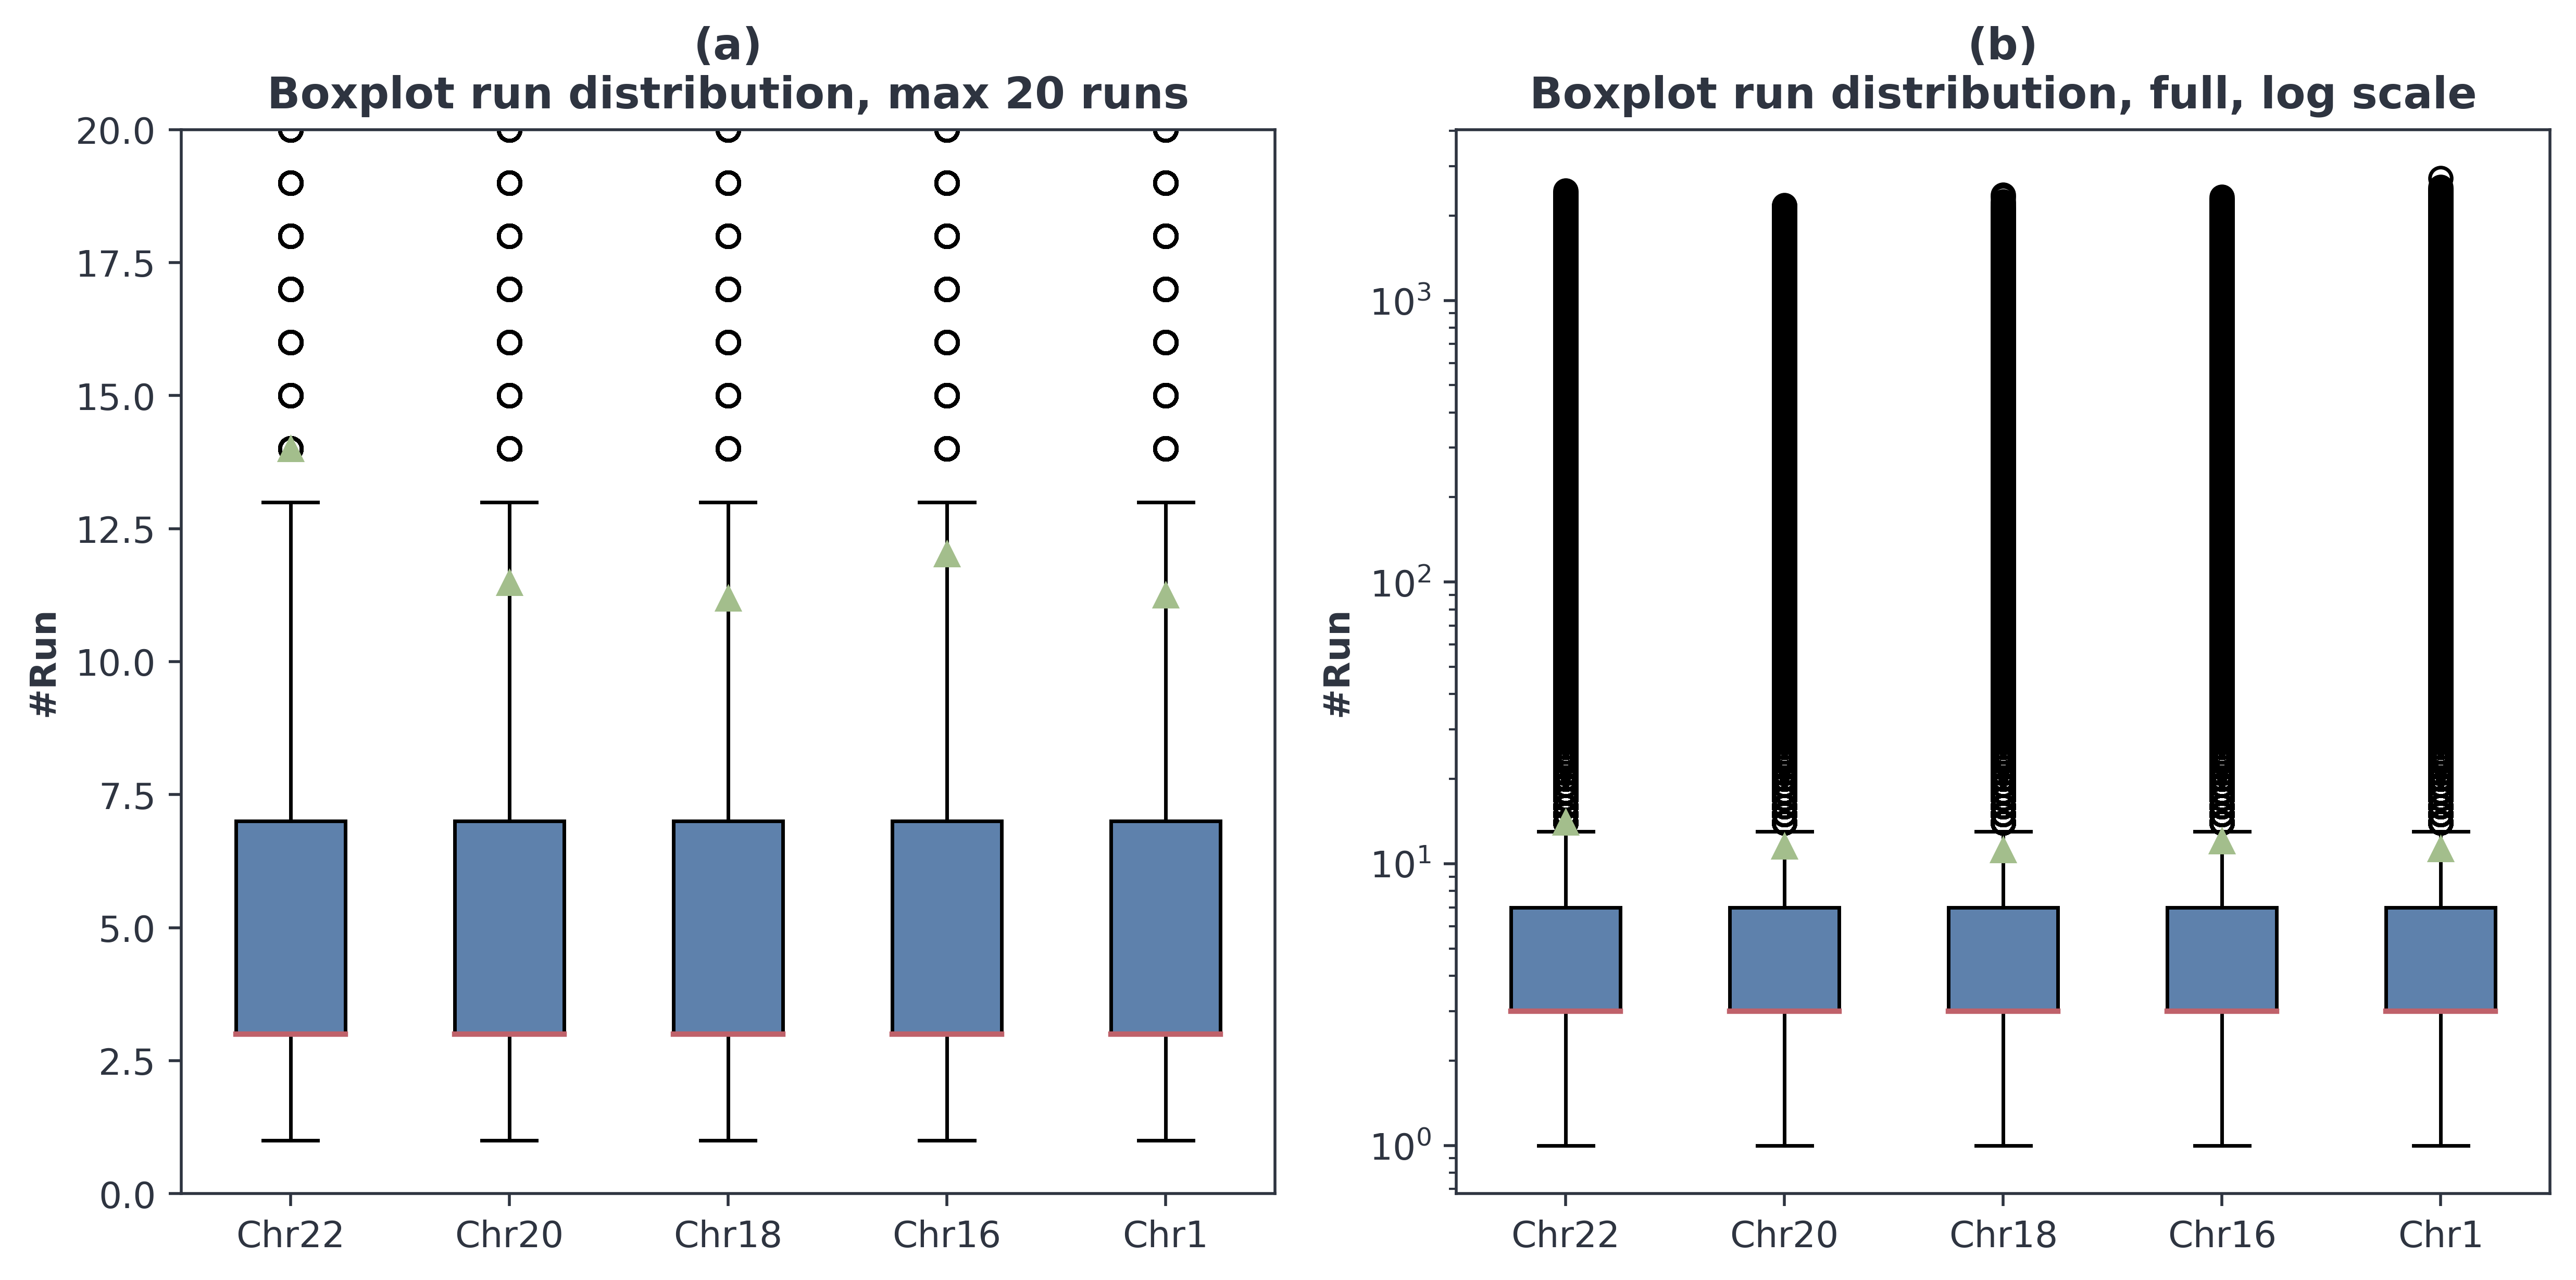
\includegraphics[width = \linewidth]{img/boxplotbi.png}
  \caption{Boxplot della distribuzione delle run per i pannelli dei cinque
    cromosomo studiati. Il grafico (a) presenta uno zoom che esclude la maggior
    parte degli outlier mentre il grafico (b) presenta, in scala logaritmica, il
    boxplot completo con tutti gli outlier.}
  \label{fig:boxplot}
\end{figure}
\subsection{Riproducibilità degli esperimenti}
Al fine di rendere riproducibili gli esperimenti, si è costruita una pipeline
per l'esecuzione dei vari algoritmi e l'estrazione dei dati quantitativi
relativi alle performance.\\
L'intera pipeline è stata gestita tramite \textbf{Snakemake} \cite{snakemake},
un \textit{workflow management system}, uno strumento molto usato in
\textit{bioinformatica} per creare analisi dati scalabili e riproducibili. Nel
dettaglio la pipeline comprende, come visualizzabile in figura \ref{fig:snake},
avendo in input un pannello ed una lista di 
quantità di aplotipi di query:
\begin{itemize}
  \item scaricamento dei tool e delle loro dipendenze per la \textit{PBWT} di
  Durbin e la \textit{RLPBWT} proposta in questa tesi
  \item produzione dell'input per la \textit{PBWT} e della \textit{RLPBWT} per
  ogni quantità di query richiesta
  \item produzione delle strutture dati
  \item esecuzione degli algoritmi per il calcolo degli \textit{SMEM}
  % \item produzione di vari grafici relativi sia ai tempi di esecuzione che alla
  % memoria richiesta
\end{itemize}
Al fine di ottenere risultati non banali, si è deciso di partire da
un pannello iniziale fisso ed estrarre un numero di righe pari al numero di
query richieste, righe che, a loro volta, andranno a formare il pannello di
query.\\
\begin{figure}
  \centering
  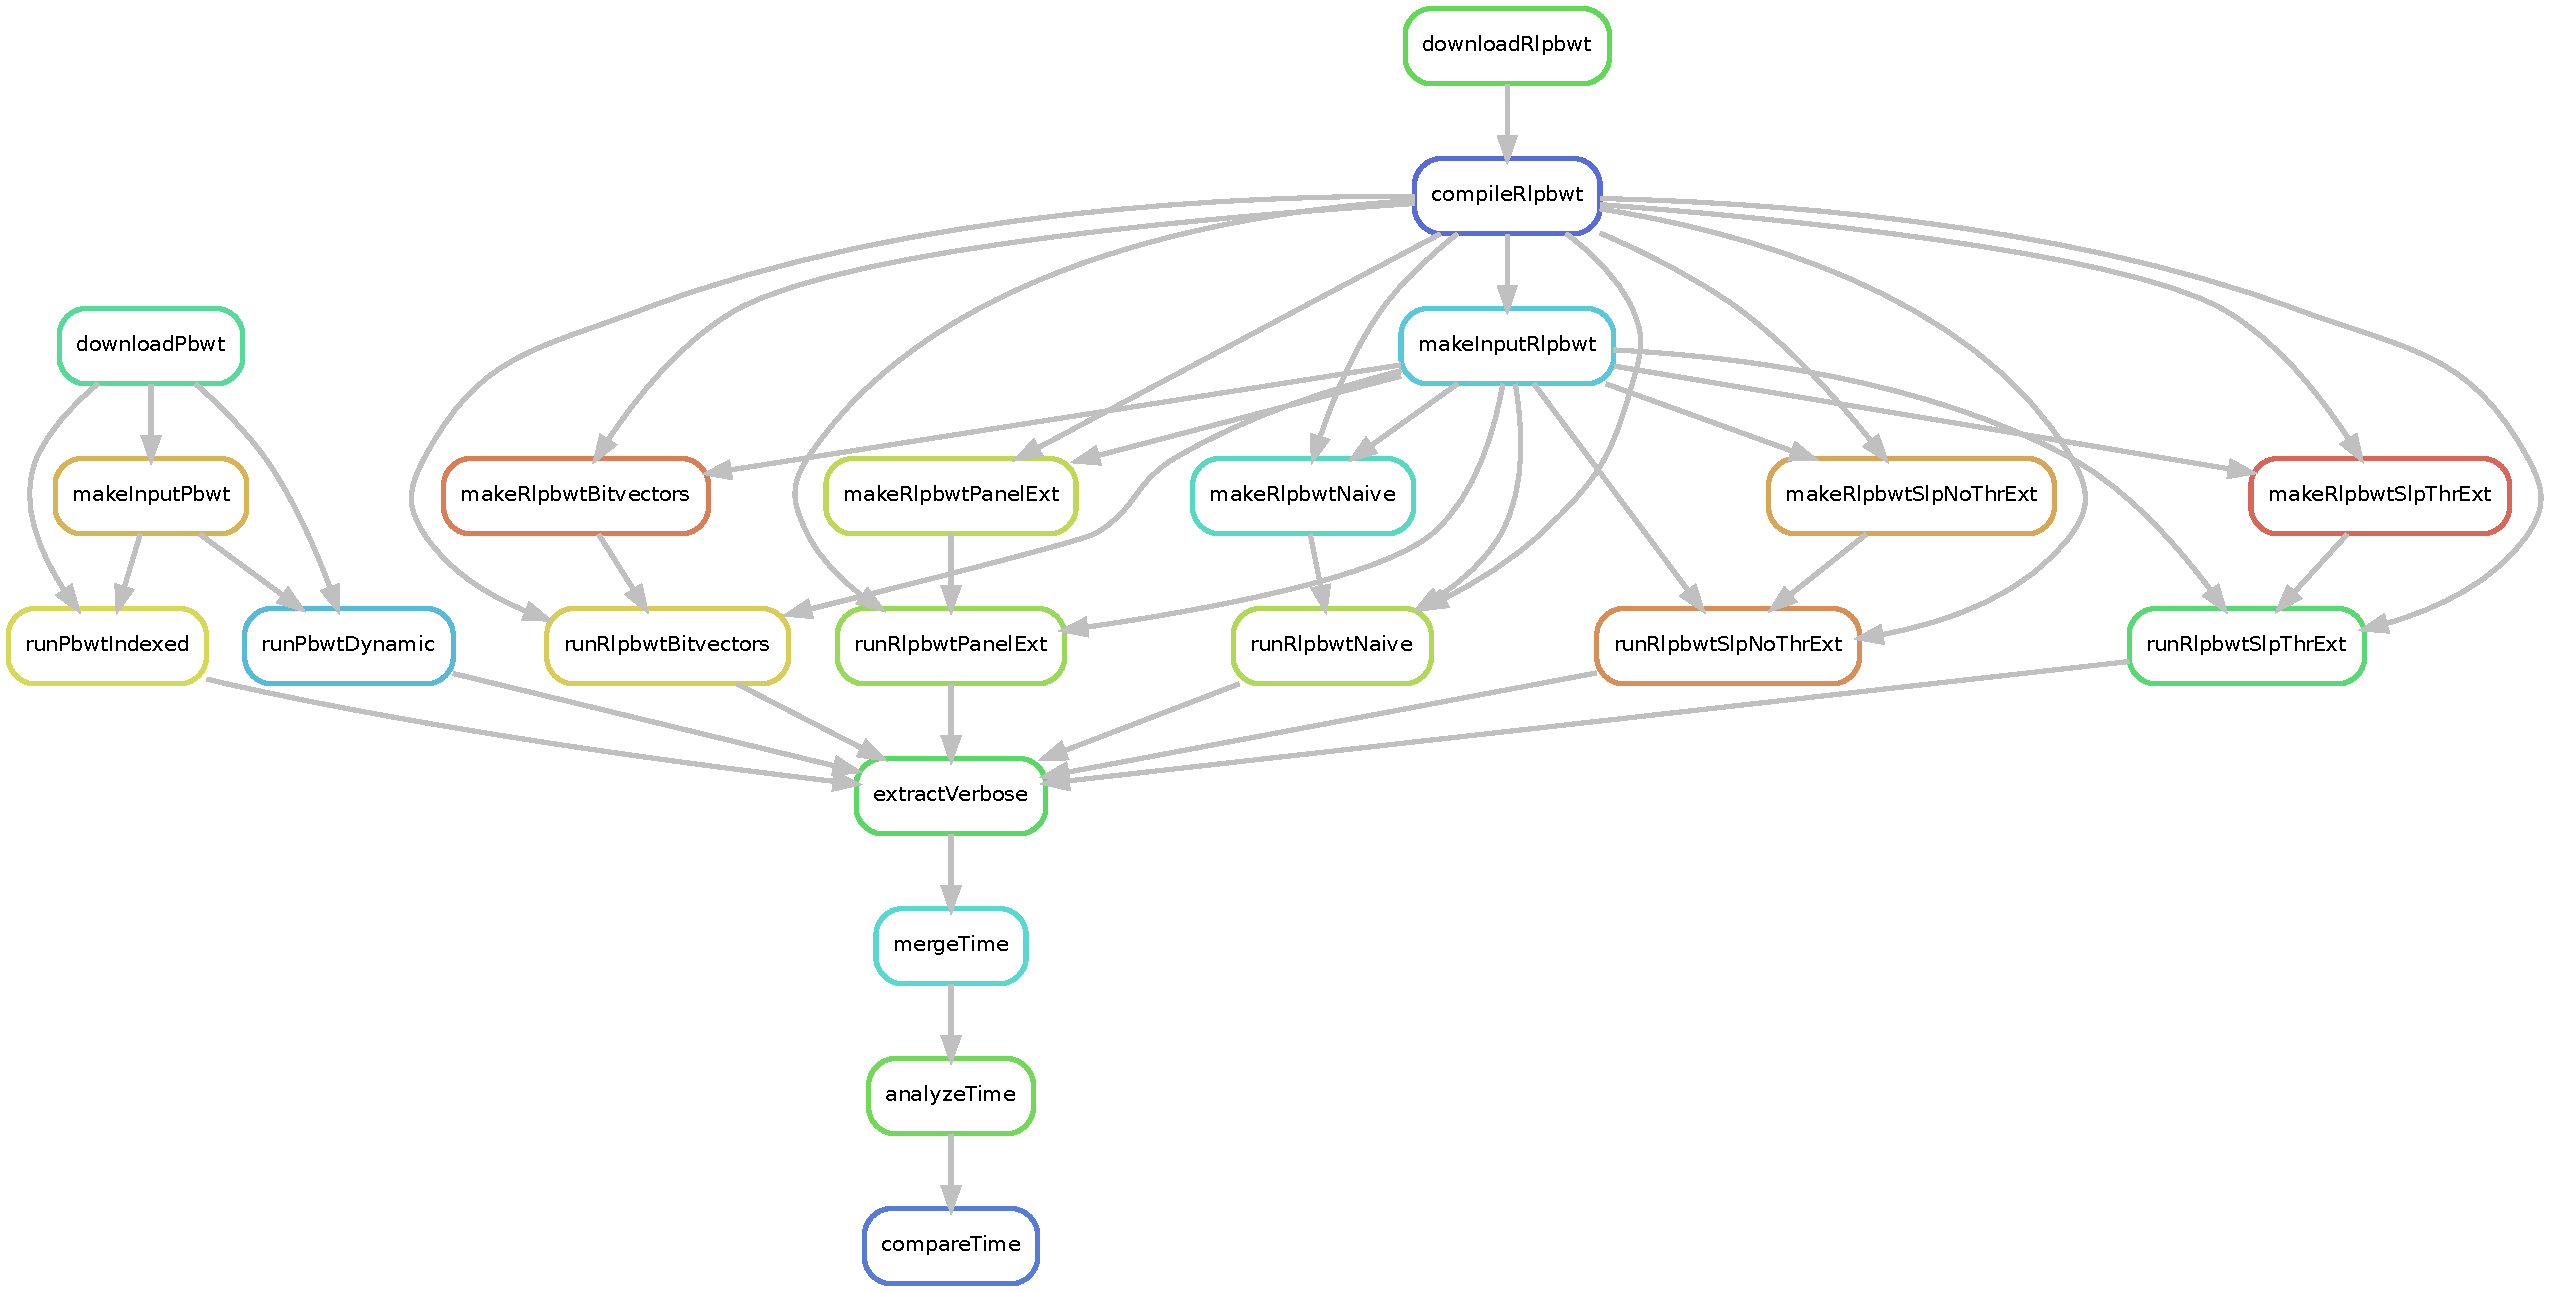
\includegraphics[width=\textwidth]{img/rules.pdf}
  \caption{Regole usate in Snakemake per la sperimentazione.}
  \label{fig:snake}
\end{figure}
\newline
\textit{La sperimentazione è stata effettuata su una macchina con processore
  Intel Xeon E5-2640 V4 ($2.40$ GHz), $756$ GB di RAM, $768$ GB di swap e
  sistema operativo Ubuntu 20.04.4 LTS. Tale macchina è stata gentilmente messa
  a disposizione dalla \emph{University of Florida}.}